\documentclass[a4paper, 12pt,oneside]{article} 
%\documentclass[a4paper, 12pt,oneside,draft]{article} 

\usepackage{preamble}
\usepackage{bm}
%--------------------- ACTUAL FILE ---------------------- %
\begin{document} 
%%%
	%\thispagestyle{empty}
	%\vspace*{\fill}
	\begin{center}
	    \Large
	    \textbf{Orthogonalization Techniques for a Set of Vectors}
	        
	    \vspace{0.4cm}
	    \large
		HPC for numerical methods and data analysis \\
	    Student : Tara Fjellman \\
	    \small{Fall 2024}
	\end{center}
	\section{Introduction}
	QR factorization is a fundamental operation in numerical linear algebra. It is used in many applications, such least squares problems, computing the low rank approximation of a matrix, and computing an orthogonal basis of a set of vectors. Its ``thin''-$Q$ version is defined as the factorization of a matrix ${A}\in \mathbb{R}^{m \times n}$ into the product of an orthogonal matrix ${Q}\in {R}^{m \times n}$ and an upper triangular matrix ${R}\in \mathbb{R}^{n \times n}$, such that ${A} = {Q} {R}$. The QR factorization can be computed using different algorithms, such as Classical Gram-Schmidt (CGS), Cholesky QR (CQR), and Tall-Skinny QR (TSQR). These algorithms have different stability properties and computational costs, which makes them suitable for different applications. In this project, we study the numerical stability and computational performance of these algorithms for orthogonalizing a set of vectors. We compare the algorithms using theoretical analysis and numerical experiments on two different matrices : a well conditioned one, and an ill-conditioned one. The goal is to identify an algorithm that is numerically stable and computationally efficient for orthogonalizing a set of vectors.
	\section{Algorithms}
		In this section we present the three algorithms that we will be considering in the study. We focus on understanding how the work and their assumptions (when it applies). 
		\subsection{Classical Gram-Schmidt}
			Given a set of linearly independent vectors $A_1, \ldots, A_n \in \mathbb{R}^m$, the Gram-Schmidt algorithm computes an orthogonal basis of size $n$,  $Q_1, \ldots, Q_n \in \mathbb{R}^m$ by orthogonalizing the $A_i$ vectors one by one. At the step $i$ of the algorithm, $A_i$ is projected onto the orthogonal complement of the space spanned by the previous vectors $Q_1, \ldots, Q_{i-1}$, and the resulting vector is normalized to obtain $Q_i$.
			CGS is obtained by approximating the projector $I-Q(:,1:i)Q^\dagger(:,1:i)$ by $I-Q(:,1:i)Q^T(:,1:i)$. This corresponds to assuming $[Q(:,1:i)^TQ(:,1:i)]^{-1}=I$, i.e. that no numerical errors are committed during the orthogonalisation process. 
		\subsection{Cholesky-QR}
			The Cholesky decomposition of a matrix ${G\in \mathbb{R}^{n\times n}}$ is a factorization of the form ${G} = {L} {L}^T$, where ${L}\in\mathbb{R}^{n\times n}$ is a lower triangular matrix.
			The CQR algorithm consists in computing $Q=AR^{-1}$ with $R$ found with help of the Cholesky decomposition of $A^TA$. Indeed, the Cholesky decomposition $A^TA=LL^T$ gives $R=L^T$ since $(QR)^T(QR)=R^TR\iff Q^TQ=I$. 
			
			Notice that in practice, instead of inverting $R$ we can solve for each column of $A^T$ the system associated to $R^TQ^T=A^T$ taking advantage of the triangular structure of $R$.
		\subsection{Tall-skinny QR}
		%Remember that communication refers to messages between processors. In the recent years we've seen trends causing floating point to become faster than communication. This is why it's important to minimize communication when dealing with parallelism.
		TSQR is a communication avoiding algorithm for matrices with many more rows than columns. 
		To better understand how it works, we first explain it assuming the matrix $A\in\mathbb{R}^{m\times n}$ is scattered row wise in 4 parts $A_0, A_1, A_2, A_3 \in \mathbb{R}^{m / 4 \times n}$. We will then explain how to generalise to the more general case. 
		
		The computation can be expressed as a product of intermediate orthonormal factors in a binary tree like structure.
		At the leaves of the binary tree, we consider the 4 local QR factorizations $A_0=\hat{Q}_0^{(2)} \hat{R}_0^{(2)}, A_1=\hat{Q}_1^{(2)} \hat{R}_1^{(2)}, A_2=\hat{Q}_2^{(2)} \hat{R}_2^{(2)}, A_3=\hat{Q}_3^{(2)} \hat{R}_3^{(2)}$. Here $\hat{Q}_l^{(2)} \in \mathbb{R}^{m / 4 \times m / 4}$ and $\hat{R}_l^{(2)} \in \mathbb{R}^{m / 4 \times n}$. As we only are interested in the thin $Q$ factor for this application, we can work with the $Q_i^{(k)}\in\mathbb R^{m/4\times n}, R_i^{(k)}\in\mathbb R^{n\times n}$ instead of the full $\hat Q_i^{(k)}, \hat R_i^{k}$ ones. We can therefore re-write these first QR factorisations in block structure as 
		$$
		\left[\begin{array}{l}
		A_0 \\
		A_1 \\
		A_2 \\
		A_3
		\end{array}\right]=\left[\begin{array}{llll}
		{Q}_0^{(2)} & & & \\
		& {Q}_1^{(2)} & & \\
		& & {Q}_2^{(2)} & \\
		& & & {Q}_3^{(2)}
		\end{array}\right]\left[\begin{array}{l}
		{R}_0^{(2)} \\
		{R}_1^{(2)} \\
		{R}_2^{(2)} \\
		{R}_3^{(2)}
		\end{array}\right].
		$$
		In the second level of the binary tree we combine the upper triangular matrix $R_0^{(2)}$ with $R_1^{(2)}$ and $R_2^{(2)}$ with $R_3^{(2)}$ to get block structured matrices. We then consider the QR factorizations to get $Q_{00}^{(1)},Q_{10}^{(1)},R_0^{(1)},Q_{22}^{(1)},Q_{32}^{(1)},R_2^{(1)}$ such that
		$$
		\left[\begin{array}{c}
		R_0^{(2)} \\
		R_1^{(2)}
		\end{array}\right]=\left[\begin{array}{c}
		{Q}_{00}^{(1)} \\
		{Q}_{10}^{(1)} 
		\end{array}\right]
		R_0^{(1)},
		\quad\left[\begin{array}{c}
		R_2^{(2)} \\
		R_3^{(2)}
		\end{array}\right]=\left[\begin{array}{c}
		{Q}_{22}^{(1)} \\
		{Q}_{32}^{(1)}
		\end{array}\right]
		R_2^{(1)}.
		$$
		This can be written as
		$$
		\left[\begin{array}{c}
		{R}_0^{(2)} \\
		{R}_1^{(2)} \\
		{R}_2^{(2)} \\
		{R}_3^{(2)}
		\end{array}\right]=\left[\begin{array}{ccc}
			{Q}_{00}^{(1)} & & \\
			{Q}_{10}^{(1)} & & \\
			& & {Q}_{22}^{(1)} \\
			& & {Q}_{32}^{(1)} 
		\end{array}\right]\left[\begin{array}{c}
		R_0^{(1)} \\
		R_2^{(1)}
		\end{array}\right].
		$$
		Finally at the root of the tree we compute the last QR factorization
		$$
		\left[\begin{array}{c}
		R_0^{(1)} \\
		R_2^{(1)}
		\end{array}\right]=\left[\begin{array}{c}
			{Q}_{00}^{(0)} \\
			{Q}_{20}^{(0)}
		\end{array}\right]
		R_0^{(0)},
		$$
		after which one can write ${Q}=Q^{(2)}Q^{(1)}Q^{(0)}$.

		In the more general case, where $A$ is distributed in $2^P$ parts, we would have $P+1$ levels in the binary tree. The $Q^{(P)}$ matrix would still be block diagonal, but with $P$ blocks of size $m/P\times n$. The other $Q^{(q)}, q=P-1,...,0$ matrices would also be block diagonal, composed of $2^q$ blocks, each of size $2n\times n$. 
		The reduction tree used was obtained at every step $q$ with the following procedure :
		(a) parts $i$ such that $i\mod 2^{P-q}=0$ are kept active; (b) part $j$ for which $j\mod 2^{P-q+1}=1$ sends data to part $i=j-2^{P-q}$; (c) part $i$ receives data from part $j=i+2^{P-q}$. This method nicely generalises the reduction tree used above for the 4 part example. 
		\subsection{Stability comparison}
		\begin{wraptable}[9]{r}{0.5\textwidth}
			\centering
			\vspace{-3em}
			\begin{tabular}{|c|c|c|}
			\hline
			\bf{Algorithm}   & $\mathbf{\|I-Q^TQ\|}$ & \bf{Constraint}  \\ \hline
			CQR & $\mathcal{O}(\varepsilon)\kappa^2(A)$  & $\mathcal{O}(\varepsilon)\kappa^2(A)<1$   \\  \hline
			CGS & $\mathcal{O}(\varepsilon)\kappa^2(A)$ & $\mathcal{O}(\varepsilon)\kappa^2(A)<1$ \\ \hline
			TSQR & $\mathcal{O}(\varepsilon)$  & None \\ \hline
			\end{tabular}
			\caption{Stability information for the considered algorithms. This data comes from the slides of the class.}
			\label{tab:stability-comparison}
		\end{wraptable}
		In this section we compare the theoretical stability of the three algorithms. We do so in terms of the loss of orthogonality $\left\|I-Q^T Q\right\|$ and the condition number of the input matrix $A$. The results are presented in \ref{tab:stability-comparison}.

		Looking at the table we can see that TSQR should by far be the most stable algorithm, as its loss of orthogonality is independent of $A$'s condition number. This makes TSQR unconditionally stable. In contrast, CGS and CQR have a loss of orthogonality that grows quadratically with the condition number of $A$. This means that for ill conditioned matrices these algorithms will be inaccurate. The condition for the algorithms to be stable is written as $\mathcal{O}(\varepsilon)\kappa^2(A)<1$, so problems should emerge for $\kappa(A)$ around $10^7$-$10^8$. 
	\section{Parallelisation}
		For parallelization of all the considered algorithms, the matrix ${A}$ is row-distributed over the cores. Each core $i=0,...,P-1$ owns a block ${A}_i$.
		
		In the following sections, parallel versions of the considered algorithms are presented with help of the pseudo-codes provided by the professor during the lectures. A comparison of computational cost is also made.
		\subsection{Classical Gram-Schmidt}
			The pseudocode for parallel CGS is given in \ref{fig:CGS-pseudocode}.   
			Parallel CGS splits the projection of the $i$th vector across the cores. This requires an Allreduce operation for every column, as the projection involves the full columns of $Q$. Indeed, to know how well two vectors align, one should sum their alignments (i.e. dot product) in every subspace. The norm of the obtained projection is also Allreduced to compute the normalization factor, which is needed across cores. After the loop is done, the final $Q$ matrix is obtained by a Gather operation.
			\begin{figure}[htb]       
				\centering             
					\vspace{0em}
					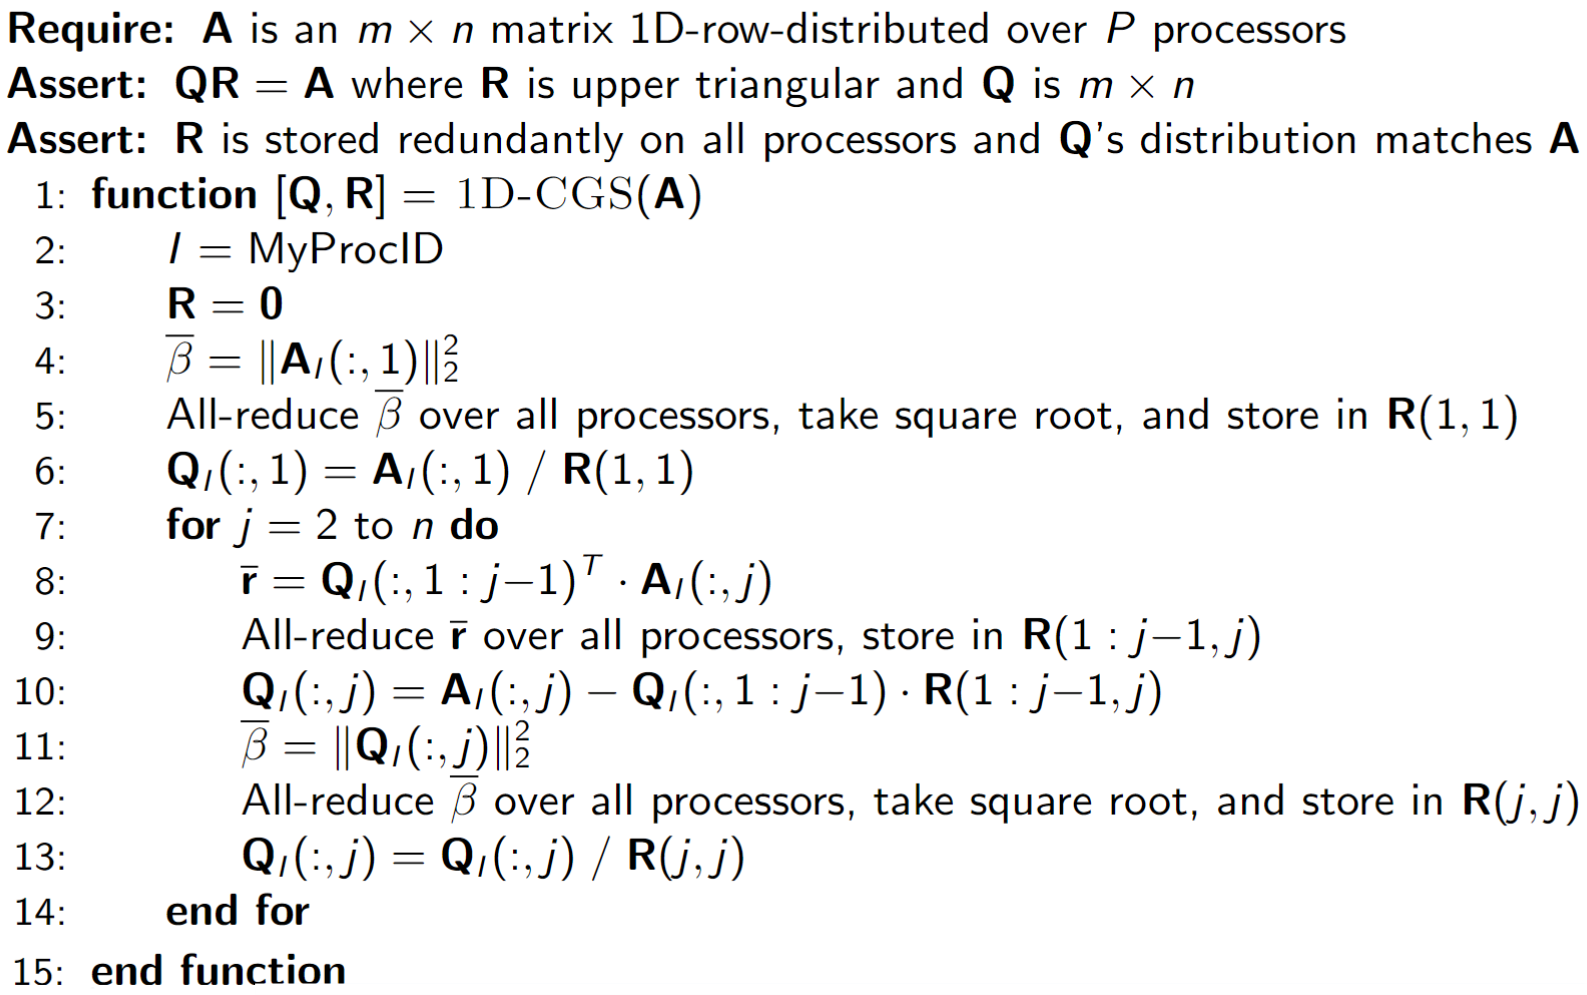
\includegraphics[width=.75\textwidth]{CGS_pseudocode}
					\caption{Pseudocode of parallelised CGS algorithm.}
					\label{fig:CGS-pseudocode}
			\end{figure}
		\subsection{Cholesky-QR}
			The pseudocode for parallel CQR is given in \ref{fig:Cholesky-QR-pseudocode}.
			Parallel CQR computes on every processor the $n\times n$ component $A_i^TA_i$ of $A^TA$. This is done by computing the local $A_i^TA_i$ and then summing the results with an Allreduce operation. The Cholesky decomposition is then computed on every processor as it is on a $n\times n$ matrix, and we want to limit unnecessary communication. The contribution $Q_i$ of processor $i$ to the $Q$ matrix is then computed by solving the system $R^TQ_i^T=A_i^T$. The final result is obtained by a Gather operation. 
			\begin{figure}
				\centering
				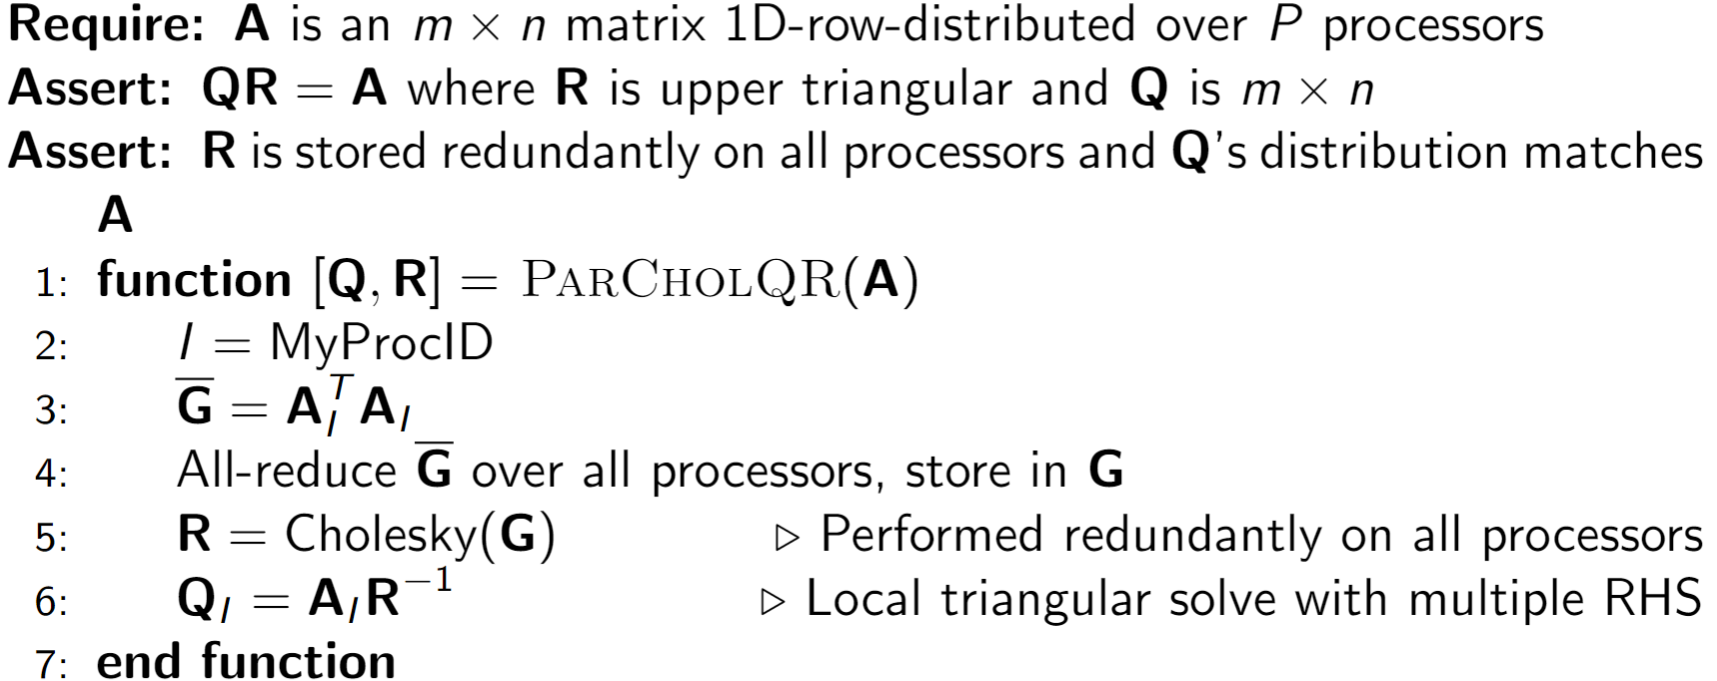
\includegraphics[width=.7\textwidth]{cholesky_QR_pseudocode}
				\caption{Pseudocode of parallelised CQR algorithm.}
				\label{fig:Cholesky-QR-pseudocode}
			\end{figure}
		\subsection{Tall-skinny QR}
			The pseudocode for TSQR is given in \ref{fig:TSQR-pseudocode}.
			TSQR was mostly explained already in the previous section. Indeed, get instruction on how to run it in parallel, one only needs to change ``part'' in ``core'' in the presentation section. We might add that the reconstruction of the $Q$ matrix is done a posteriori by building the $Q^{(k)}$ matrices going up the binary tree and multiplying it by the trailing $Q^{(k-1)\leftarrow(0)}:=Q^{(k-1)}...Q^{(0)}$ matrix. 
			% 	In this project we consider $m \gg n$ and typically take $n$ between 50 and a few hundreds, while $m$ can be much larger.
			\begin{figure}
				\centering
				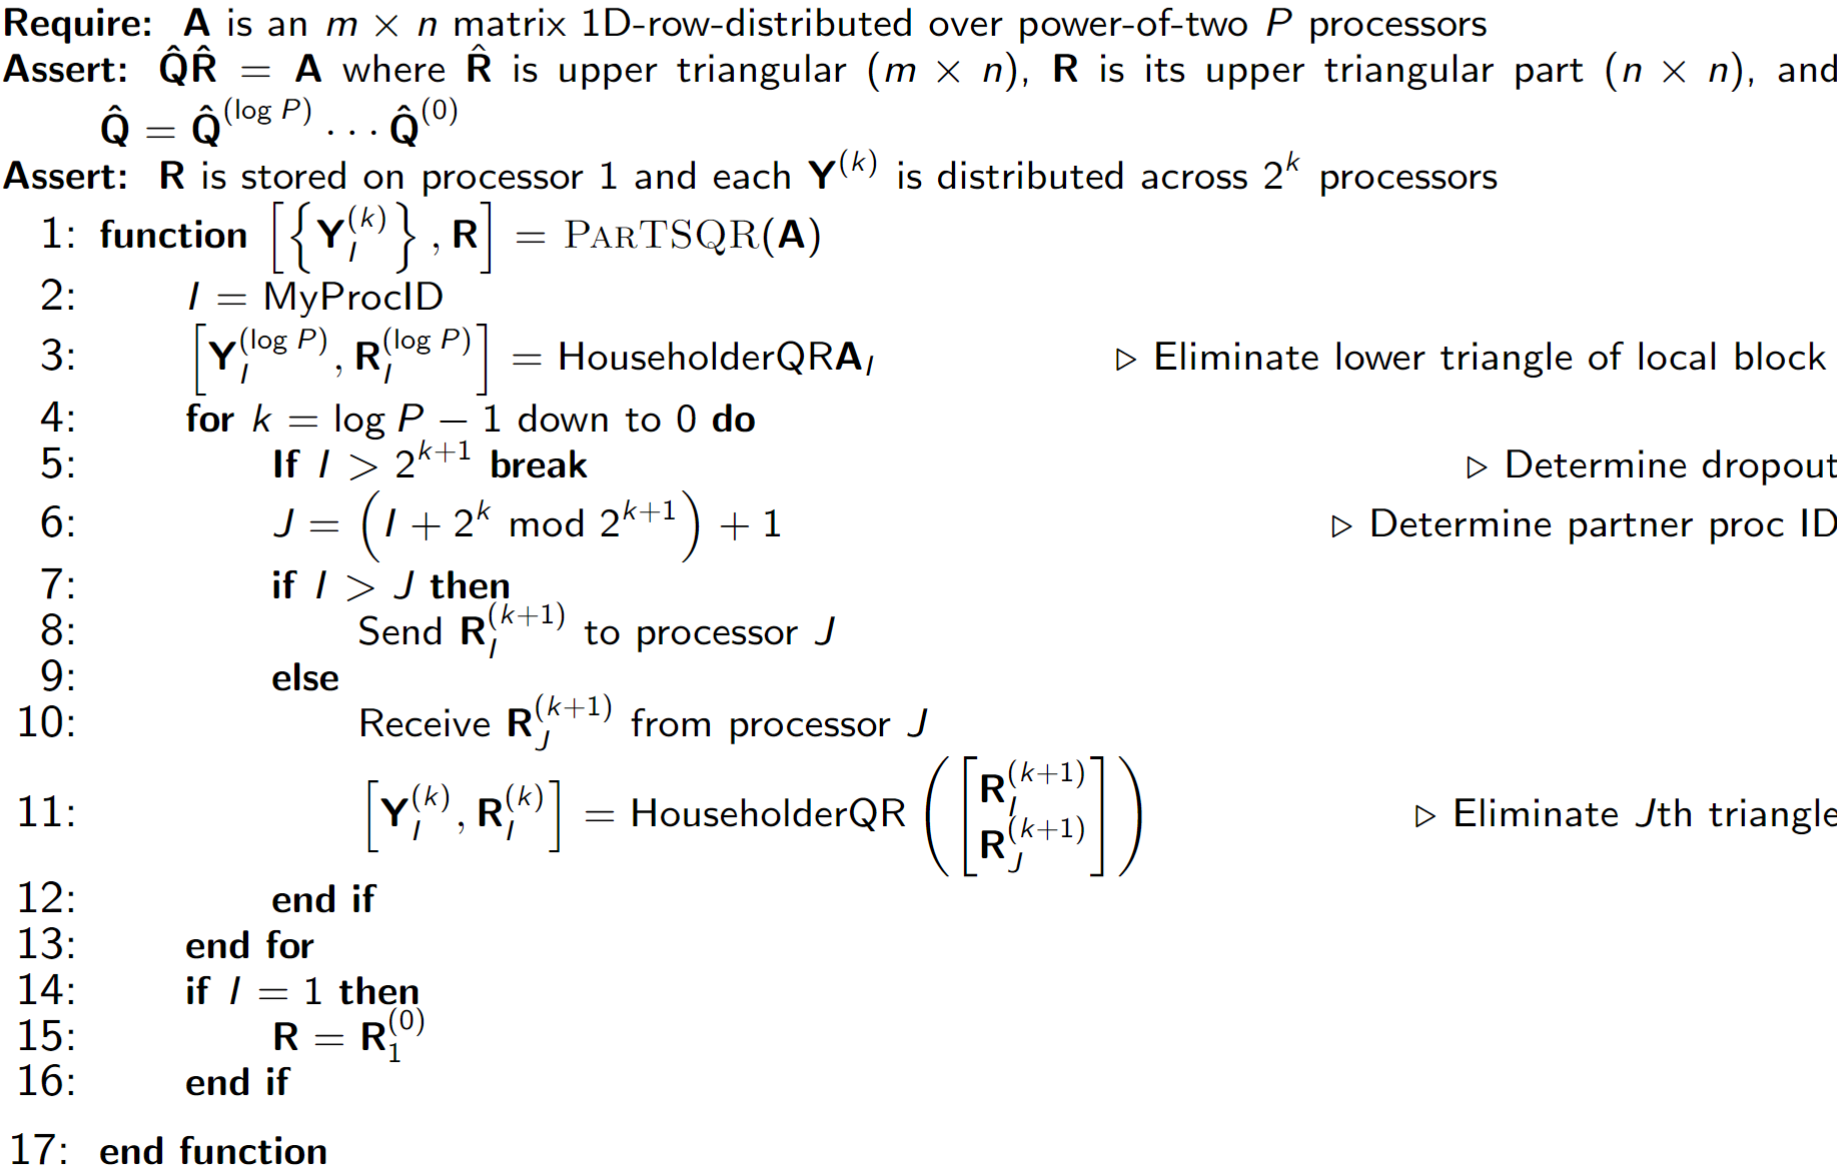
\includegraphics[width=.8\textwidth]{TSQR_pseudocode}
				\caption{Pseudocode of parallelised TSQR algorithm.}
				\label{fig:TSQR-pseudocode}
			\end{figure}
		\subsection{Cost comparison}
		\begin{table}
			\centering
			\vspace{-1em}
			\begin{tabular}{|c|c|c|c|}
			\hline
			\bf{Algorithm}   & \bf{\# FlOps} & \bf{\# Words} & \bf{\# Messages}  \\ \hline
			CGS & $2mn^2/P$  & $\mathcal{O}(n^2 + n\log_2 P)$ & $\mathcal{O}(n\log_2 P)$  \\  \hline
			CQR &  $2mn^2/P + n^3/3$ & $\mathcal{O}(n^2)$ & $\mathcal{O}(\log_2 P)$ \\ \hline
			TSQR &  $2mn^2/P + 2n^3/3 \times \log_2 P$  & $\mathcal{O}(n^2\log_2 P)$ & $\mathcal{O}(\log_2 P)$ \\ \hline
			\end{tabular}
			\caption{Information about computational cost of the considered algorithms. This data comes from the slides of the class. The values assume $P<m/n$, and those of CQR further assumes $P\leq n^2$.}
			\label{tab:cost-comparison}
		\end{table}
		In this section we compare the theoretical computational costs of the three algorithms. We do so in terms of the required number of floating point operations, sent messages and sent words. The results are presented in \ref{tab:cost-comparison}.

		Looking at the table it is clear that CGS has the highest communication cost, as it requires $n$ Allreduce operations (one for every column). This is in contrast to CQR and TSQR, which do not require any data duplication. These algorithms actually are communication optimal. 

		The number of floating point operations is similar for all algorithms, as the dominating term is $2mn^2/P$ each time. TSQR and CQR have an $\mathcal{O}(n^3)$ term due to respectively : the Householder QR decompositions of the $2n\times n$ matrices; the Cholesky decomposition of an $n\times n$ matrix.
	\section{Experimental procedure}
		For all the presented results, we used $m=2^{15}=32768$ and $n=330$, unless stated otherwise. This choice was based on the fact that we wanted the computations of the metrics to take a reasonable time, while providing the algorithms with a sufficiently large matrix for the run times not to have too high of a variance.	
		\subsection{Chosen Matrices}
			The ill conditioned matrix, which we denote $C \in \mathbb{R}^{m \times n}$ was generated by uniformly discretizing the following parametric function
			$$
			f(x, y)=\frac{\sin [10(y+x)]}{\cos [100(y-x)]+1.1},
			$$
			over the $0 \leq x, y \leq 1$ domain.

			The well conditioned matrix was obtained from the SuiteSparse Matrix Collection [1]. More precisely, a $50000\times 50000$ matrix was used. To make it $m\times n$, its first $m$ lines and $n$ columns were kept. 
		\subsection{Numerical Stability}
			For the numerical investigation, the loss of orthogonality is measured as $\left\|I-Q^T Q\right\|$ and the condition number of the basis $Q$. Indeed, the condition number of the basis $Q$ is also a measure of orthogonality since it is defined as the ratio of the largest and smallest singular values $\sigma_{\max{}},\sigma_{\min}$ of $Q$ and orthogonal matrices should have $|\sigma_i|=1\ \forall i$. 
		
			In general, these quantities where considered for the whole matrix $Q$, end of the algorithm. For CGS, however, as it is possible and relevant, an analysis of these quantities' evolution over the iterations of the algorithm when was also led (so considering $Q(:,1:j)$ for $j=1,...,n$).

			% message zayneb
			Also, CQR could not be run on big $C$ matrices due to numerical stability issues. Indeed, the function for the Cholesky decomposition perceived these matrices as being singular (up to machine precision). We therefore studied its behaviour as a function of matrix size for smaller sizes. This was done by considering the $C_s=C(m=2000s,5s)$ matrix for values of $s$ between 1 and 30, which made the condition number of $C_s$ vary from $10^1$ to $10^7$.
		\subsection{Runtimes}
			All the presented results where run on the Helvetios cluster. On this cluster, each node is composed of 2 Skylake processors running at 2.3 GHz, with 18 cores each [2]. For the results to be easily interpretable, only one core per task was used.

			The run times where obtained by timing each active core $i$, and then taking the $\max{}$ over these, to obtain the effective run time of the computation. To quantify uncertainty and get a more accurate estimate, the run times were measured by repeating the computations $n_{\text{rep}}=5$ times.
			The number of cores was varied by taking powers of 2 between 1 and 64.

			In the code, the run times for TSQR where obtained by ignoring the construction duration, as the code for it was not optimised. Not to bias the results in favour of this algorithm, these run times were multiplied by 2 as an efficient implementation of the construction takes a similar time to that of TSQR itself [3].  	
	\section{Numerical Stability Investigation}
		\subsection{CGS as a function of $n$}
		\begin{wrapfigure}[32]{r}{0.525\textwidth}
			\vspace{-1em}
			\centering
			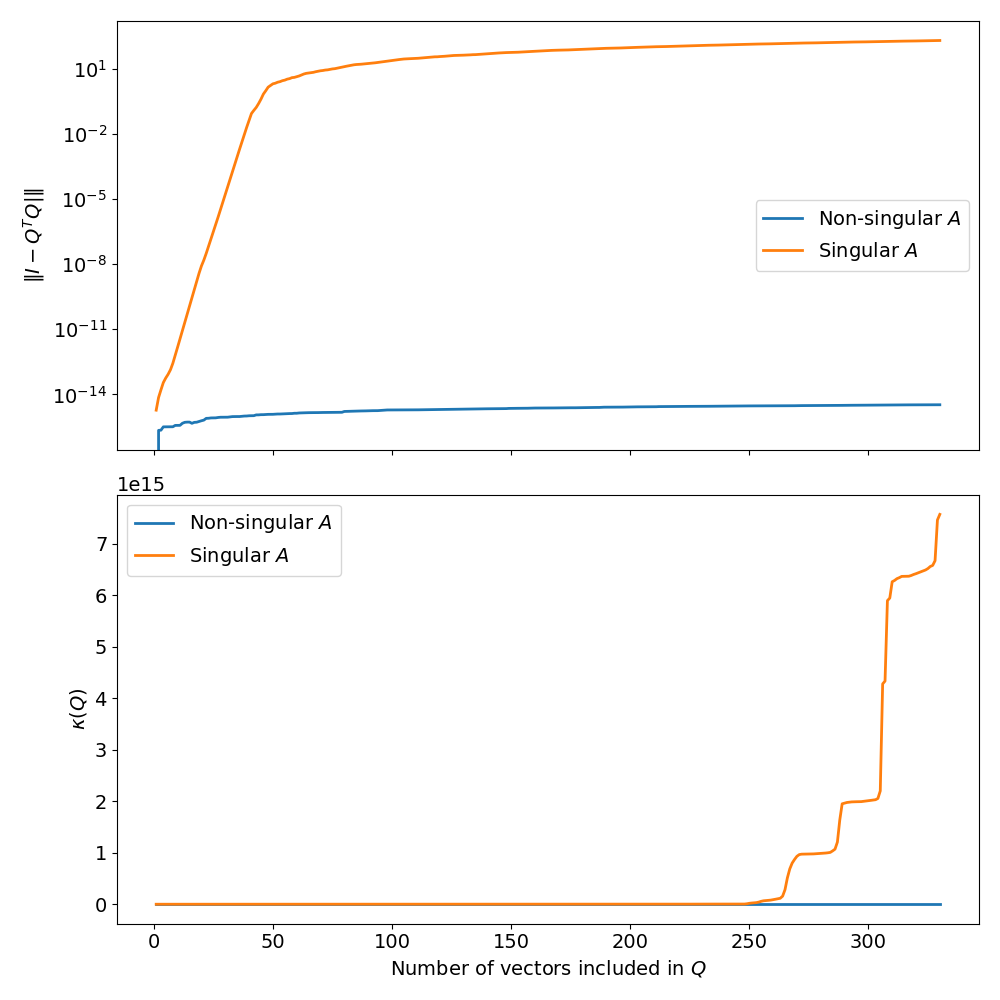
\includegraphics[width=.5\textwidth]{CGS_metric_evolution}
			\caption{Evolution of orthogonality metrics for CGS as a function of $n$.}
			\label{fig:CGS-metric-evolution}
		\end{wrapfigure}
		The first thing we explore is the behaviour of the loss of orthogonality and condition number of the $Q$ matrix as a function of the number $n$ of vectors that are added to the orthogonal basis. To do this, the metrics are computed for $n$ between 1 and 330, and the results are plotted on semi-log plots in \ref{fig:CGS-metric-evolution}.

		Looking at these plots, we see that both metrics explode as a function on $n$ for the ill conditioned matrix. The loss of orthogonality actually behaves exponentially for small values of $n$ (i.e. up to $\sim 50$ or so), before plateauing at a value of order 100. Both these behaviours can be understood as follows. (1.) The $n$th added vector needs to be orthogonal to $n-1$ other ones, and so contributes to $n-1$ numerical errors. (2.) The vectors are normed to $1$ and so the loss of orthogonality plateaus to a value similar to that characteristic of some random matrix under the same constraint. 

		For the well conditioned matrix, the loss of orthogonality quickly plateau at value which is not far from machine precision. This is expected, as the condition number of the matrix is much lower, and therefore $\mathcal{O}(\varepsilon)\kappa^2(A)\ll 1$.

		The condition number for the ill conditioned matrix has a more surprising curve. Indeed, there seem to be some really small plateaus whose structure repeats periodically with period $\sim 40$. I was not able to come up with a good explanation for this behaviour. Another interesting point to notice is that the condition number starts to increase only once the loss of orthogonality has exploded. This was, at least partly expected, as singular values of an orthogonal matrix are 1. Notice that for the well conditioned matrix, the condition number is always 1, as expected. 
		%\lipsum[1-4]
		\subsection{Algorithm comparison}
		We now compare the three algorithms between them. We do so by considering the loss of orthogonality and $Q$'s condition number at the end of the computation. The results are presented in \ref{tab:numberical-stability}.

		As a quick look to the table confirms, the observed behaviours are the expected ones. For the well conditioned matrix, all algorithms perform well, yielding a perfect condition number, and a loss of orthogonality of the order of machine precision. For the ill-conditioned matrix : TSQR performs just as well, as it is unconditionally stable; CGS gets nonsensical results, as the $Q$ matrix has a condition number of order $10^{15}$, and the loss of orthogonality saturates; while CQR runs into a fatal error, as it perceives the $A^TA$ matrix as singular.
		
		From this analysis, we can conclude that TSQR is the only algorithm one should use if dealing with ill conditioned matrices. For well-conditioned matrices, all algorithms are equivalent from the stability point of view.  
		\begin{table}[h]
			\centering
			\begin{tabular}{|c|c|c|c|c|}
			\hline
			\bf{Metric} & $\mathbf{\kappa(A)}$ & \bf{CQR} & \bf{CGS} & \bf{TSQR}  \\ \hline
			\multirow{2}{*}{$\mathbf{\|I-Q^TQ\|}$} & $1.984\times 10^{4}$  & 4.153$\times 10^{-15}$ & 3.350$\times 10^{-15}$ & 5.550$\times 10^{-15}$ \\ \cline{2-5} 
											  & $3.883\times 10^{15}$ & Error & 1.991$\times 10^{2}$ & 8.255$\times 10^{-15}$ \\ \hline
			\multirow{2}{*}{$\mathbf{\kappa(Q)}$} & $1.984\times 10^{4}$  & 1+$\mathcal{O}(\varepsilon)$ & 1+$\mathcal{O}(\varepsilon)$ & 1+$\mathcal{O}(\varepsilon)$ \\ \cline{2-5} 
											  & $3.883\times 10^{15}$ & Error & 7.572$\times 10^{15}$ & 1+$\mathcal{O}(\varepsilon)$ \\ \hline
			\end{tabular}
			\caption{Metrics for numerical stability of the considered algorithms. The entries for the ill-conditioned matrix and CQR are marked as ``Error'' as the algorithm could not be run.}
			\label{tab:numberical-stability}
			\end{table}
			\subsection{CQR's stability : a deeper look}
			\begin{wrapfigure}[18]{r}{0.55\textwidth}
				\centering
				\vspace{-3em}
				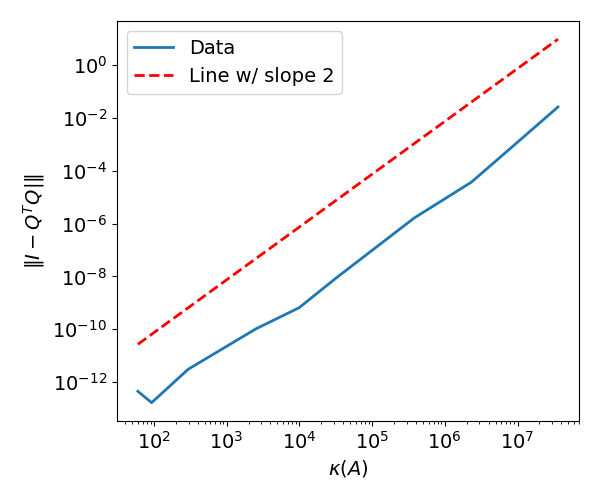
\includegraphics[width=.55\textwidth]{CQR_stability}
				\caption{Loss of orthogonality of the $Q$ matrix obtained by CQR as a function of $A$'s condition number.}
				\label{fig:CQR-stability}
			\end{wrapfigure}
			To better understand the numerical stability issues that CQR runs into, we now turn to its behaviour as a function of $A$'s condition number. The associated results are presented in a log-log plot in \ref{fig:CQR-stability}.
			Looking at the plot, we can see that the loss of orthogonality grows quadratically as a function of the condition number (the slope on a log-log plot is an exponent on a lin-lin plot). This observation is compatible with the theoretical prediction, as CQR makes use of the Cholesky decomposition of $A^TA$, which has condition number $\kappa(A^TA)=\kappa(A)^2$. This allows us to conclude that the algorithm will interpret matrices with a condition number above $10^8$ as if they where singular. This is indeed what the presented theory predicted. 
			%To better understand the Your report should state the theoretical bounds for the loss of orthogonality of the three algorithms. You should explain why these measures are important. For each matrix you should plot or put in a table the loss of orthogonality/condition number. You should explain these plots, reference them, and make connection with the theory.
	\section{Runtime Investigation}
		Note that the results for CQR are not presented for the ill-conditioned matrix, as the algorithm could not be run on it.
		\subsection{Sequential runtimes}
		We start by considering the run times of the algorithms in a sequential setting. The results correspond to the first point of every color in the plots of the next section. The results are presented in \ref{fig:runtime-vs-nprocs-mat}.
		
		Looking at the results, we immediately see that CGS and TSQR have a similar run time. This makes sense, as the two algorithms have similar number of FlOps. CQR, on the other hand, when it is able to run, seems to run more than four times as fast. This can be surprising at first given that it in principle it also has a similar number of FlOps. A reason for this could be the fact that the implementation of CQR is the one that relies the most on \texttt{numpy}, which is a very well optimized library.

		\begin{wrapfigure}[30]{r}{0.5\textwidth}
			\centering
			\vspace{-1.5em}
			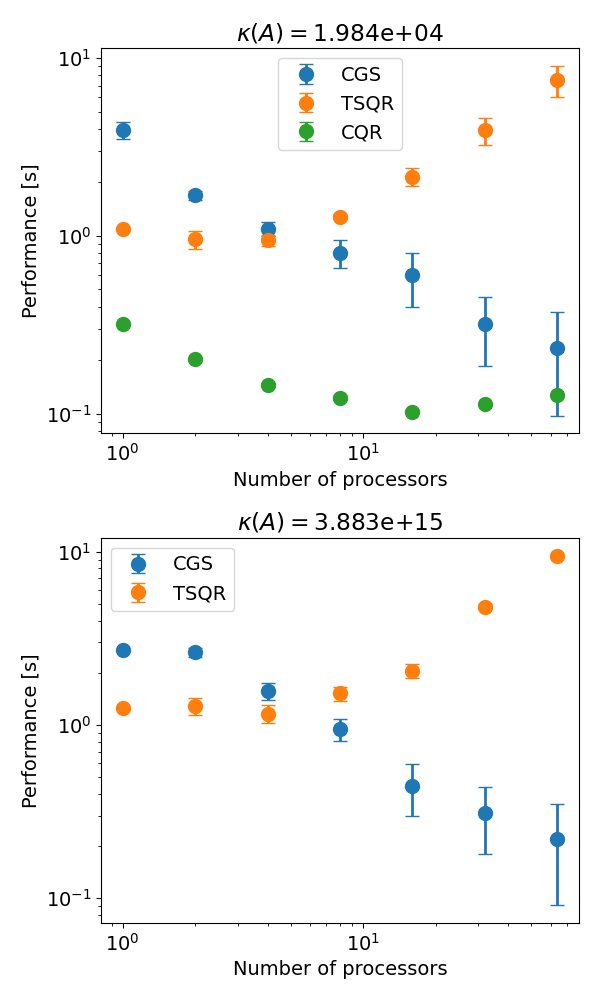
\includegraphics[width=.5\textwidth]{runtime_vs_nprocs}
			\caption{Run times for the considered algorithms, and for both well and ill conditioned matrices.}
			\label{fig:runtime-vs-nprocs-mat}
		\end{wrapfigure}
		When comparing the results for the well and the ill conditioned matrices, we see that the run times are similar (for the algorithms able to run it). 
		\subsection{Parallel runtimes}
		We now turn to the parallel run times of the algorithms. The relevant results are still those presented in \ref{fig:runtime-vs-nprocs-mat}.

		A quick look is sufficient to notice that for all algorithms, the run times decrease quasi linearly on the log-log plot for a number of cores between 1 and 8. This is a good sign, as it suggests that the algorithms are well parallelized. It is also interesting to note tha the slopes of the algorithms look similar.
		
		After this first phase, the algorithms behave differently. CGS continues to decrease steadily, TSQR plateaus, and CQR starts to increase. We know that when the number of cores increases, the cost of communication increases, while the computation time of the tasks decreases. The observed results are however still surprising given that in principle TSQR and CQR should have a better communication/computation ratio than CGS. I suspect that for bigger matrices, results closer to the theory would have been observed. Indeed, if $m/P$ is not big enough, the return of parallelisation could be limited for some algorithms.

		The maximal speed-ups are obtained for 64 cores for CGS, 32 cores for TSQR and 16 for CQR. Their values are respectively around 40, 14 and 5.5.

		Comparing the performances of CGS and TSQR between the different matrices we see that the behaviours are quite similar. Indeed, both times the same pattern of steady decrease is observed for CGS, while TSQR still saturates for more than 16 cores. There seems to be a slight difference for the speed decrease of TSQR run times however. Indeed the decrease is slightly quicker for the well conditioned matrix. This is not predicted by the theory, so the reason might be due to the matrix's specific structure (eg. by the fact that it is sparse). 
	\section{Conclusion}
	In this report we have studied the numerical stability and computational performance of three algorithms for orthogonalizing a set of vectors. After presenting the algorithms, as well as their parallelisation, we have compared the algorithms using theoretical analysis and numerical experiments on two different matrices : a well conditioned one, and an ill-conditioned one. The results show that CQR was most efficient for the well conditioned matrix, but was unable to run for matrices whose condition number surpassed $10^8$. TSQR was found to be by far the most stable algorithm, providing great results even for a matrix with condition number $~10^{15}$. Its performance for the most part matched that of CGS, meaning it should be preferred over it for ill-conditioned matrices. 
	\section*{Aknowledgements}
	I would like to thank the professor for having a Zoom call with me to clarify my questions about compact representation of $Q$ matrices in TSQR. I also thank Amal Seddas for her help in formulating and completing my questions. I also acknowledge having used github copilot to auto complete some of my coding and sentences in this report and Chat GPT to gain insight on some problems I faced along the way. I want to note that I never left the output of these tools as is, but always modified it to fit my needs and apply a critical point of view.
	\section*{References}
	[1] ‘GHS\_psdef/cvxbqp1 : SuiteSparse Matrix Collection’. Accessed: Sep. 28, 2024. [Online]. Available: https://sparse.tamu.edu/GHS\_psdef/cvxbqp1
	
	[2] ‘Helvetios’, EPFL. Accessed: Nov. 03, 2024. \newline [Online]. Available: https://www.epfl.ch/research/facilities/scitas/hardware/helvetios/
	
	[3] G. Ballard, J. Demmel, L. Grigori, M. Jacquelin, H. D. Nguyen, and E. Solomonik, ‘Reconstructing Householder Vectors from Tall-Skinny QR’, in 2014 IEEE 28th International Parallel and Distributed Processing Symposium, May 2014, pp. 1159–1170. doi: 10.1109/IPDPS.2014.120.
	%\appendix
	%	\section{Runtime Estimation}\label{appendix:runtime_estimation}
%%%
\end{document} 